\documentclass[letterpaper,12pt]{article}\usepackage[]{graphicx}\usepackage[]{color}
%% maxwidth is the original width if it is less than linewidth
%% otherwise use linewidth (to make sure the graphics do not exceed the margin)
\makeatletter
\def\maxwidth{ %
  \ifdim\Gin@nat@width>\linewidth
    \linewidth
  \else
    \Gin@nat@width
  \fi
}
\makeatother

\definecolor{fgcolor}{rgb}{0.345, 0.345, 0.345}
\newcommand{\hlnum}[1]{\textcolor[rgb]{0.686,0.059,0.569}{#1}}%
\newcommand{\hlstr}[1]{\textcolor[rgb]{0.192,0.494,0.8}{#1}}%
\newcommand{\hlcom}[1]{\textcolor[rgb]{0.678,0.584,0.686}{\textit{#1}}}%
\newcommand{\hlopt}[1]{\textcolor[rgb]{0,0,0}{#1}}%
\newcommand{\hlstd}[1]{\textcolor[rgb]{0.345,0.345,0.345}{#1}}%
\newcommand{\hlkwa}[1]{\textcolor[rgb]{0.161,0.373,0.58}{\textbf{#1}}}%
\newcommand{\hlkwb}[1]{\textcolor[rgb]{0.69,0.353,0.396}{#1}}%
\newcommand{\hlkwc}[1]{\textcolor[rgb]{0.333,0.667,0.333}{#1}}%
\newcommand{\hlkwd}[1]{\textcolor[rgb]{0.737,0.353,0.396}{\textbf{#1}}}%
\let\hlipl\hlkwb

\usepackage{framed}
\makeatletter
\newenvironment{kframe}{%
 \def\at@end@of@kframe{}%
 \ifinner\ifhmode%
  \def\at@end@of@kframe{\end{minipage}}%
  \begin{minipage}{\columnwidth}%
 \fi\fi%
 \def\FrameCommand##1{\hskip\@totalleftmargin \hskip-\fboxsep
 \colorbox{shadecolor}{##1}\hskip-\fboxsep
     % There is no \\@totalrightmargin, so:
     \hskip-\linewidth \hskip-\@totalleftmargin \hskip\columnwidth}%
 \MakeFramed {\advance\hsize-\width
   \@totalleftmargin\z@ \linewidth\hsize
   \@setminipage}}%
 {\par\unskip\endMakeFramed%
 \at@end@of@kframe}
\makeatother

\definecolor{shadecolor}{rgb}{.97, .97, .97}
\definecolor{messagecolor}{rgb}{0, 0, 0}
\definecolor{warningcolor}{rgb}{1, 0, 1}
\definecolor{errorcolor}{rgb}{1, 0, 0}
\newenvironment{knitrout}{}{} % an empty environment to be redefined in TeX

\usepackage{alltt}

\usepackage{verbatim}  % for \verbatiminput of R code
\usepackage{amsmath}  % for \eqref, and others

% define the title, author, date
\title{Stat 590 HW 1}
\author{J.R.R.~Kurtosis}
\date{\today}

%%%%%%%%%%%%%%%%%%%%%%%%%%%%%%%%%%%%%%%%%%%%%%%%%%%%%%%%%%%%%%%%%%%%%%%%%%%%%%%%
\IfFileExists{upquote.sty}{\usepackage{upquote}}{}
\begin{document}






% generates the title
\maketitle

% insert the table of contents
\tableofcontents


%%%%%%%%%%%%%%%%%%%%%%%%%%%%%%%%%%%%%%%%%%%%%%%%%%%%%%%%%%%%%%%%%%%%%%%%%%%%%%%%
\section{Introduction}
Here's the first paragraph of the section, which is not indented.
As long as you keep lines together, they'll appear in the same paragraph.
A blank line will separate paragraphs.

Here's that new paragraph, this and every following paragraph is indented.

%%%%%%%%%%%%%%%%%%%%%%%%%%%%%%%%%%%%%%%%%%%%%%%%%%%%%%%%%%%%%%%%%%%%%%%%%%%%%%%%
\section{Methods}

You can insert R code like this code chunk below, which will print the values,
  and produce a plot.
% A percent sign preceeds LaTeX comments.

% knitr code chunk options are in the <<...>>=
% Learn more here: http://yihui.name/knitr/options#chunk_options
%   echo = whether to print source code in document
%   size = size of the code text, if echoed
%   include = whether to include chunk output in document
%   fig.width = figure width in inches
%   fig.height = figure height in inches
%   out.width = scaling figure to fit on page (can be inches, or other, or relative to page size)
% Many other optios are also available!
\begin{knitrout}
\definecolor{shadecolor}{rgb}{0.969, 0.969, 0.969}\color{fgcolor}\begin{kframe}
\begin{alltt}
\hlnum{1}\hlopt{+}\hlnum{1}
\end{alltt}
\begin{verbatim}
## [1] 2
\end{verbatim}
\begin{alltt}
\hlstd{letters[}\hlnum{5}\hlopt{:}\hlnum{10}\hlstd{]}
\end{alltt}
\begin{verbatim}
## [1] "e" "f" "g" "h" "i" "j"
\end{verbatim}
\begin{alltt}
\hlstd{LETTERS[}\hlnum{11}\hlopt{:}\hlnum{15}\hlstd{]}
\end{alltt}
\begin{verbatim}
## [1] "K" "L" "M" "N" "O"
\end{verbatim}
\begin{alltt}
\hlcom{# Create a data.frame called df used for an example plot}
\hlstd{df} \hlkwb{<-} \hlkwd{data.frame}\hlstd{(}\hlkwc{x} \hlstd{=} \hlkwd{rnorm}\hlstd{(}\hlnum{100}\hlstd{))}
\hlstd{df}\hlopt{$}\hlstd{y} \hlkwb{<-} \hlstd{df}\hlopt{$}\hlstd{x} \hlopt{+} \hlkwd{rnorm}\hlstd{(}\hlnum{100}\hlstd{,} \hlkwc{mean} \hlstd{=} \hlnum{2}\hlstd{,} \hlkwc{sd} \hlstd{=} \hlnum{0.1}\hlstd{)}

\hlcom{# plot the df data.frame}
\hlkwd{library}\hlstd{(lattice)}
\hlkwd{xyplot}\hlstd{(y} \hlopt{~} \hlstd{x,} \hlkwc{data} \hlstd{= df,}
       \hlkwc{main} \hlstd{=} \hlstr{"Title is up here"}\hlstd{,} \hlkwc{sub}\hlstd{=}\hlstr{"Subtitle is down here"}\hlstd{,}
       \hlkwc{xlab}\hlstd{=}\hlstr{"x variable"}\hlstd{,} \hlkwc{ylab}\hlstd{=}\hlstr{"y variable"}\hlstd{)}
\end{alltt}
\end{kframe}
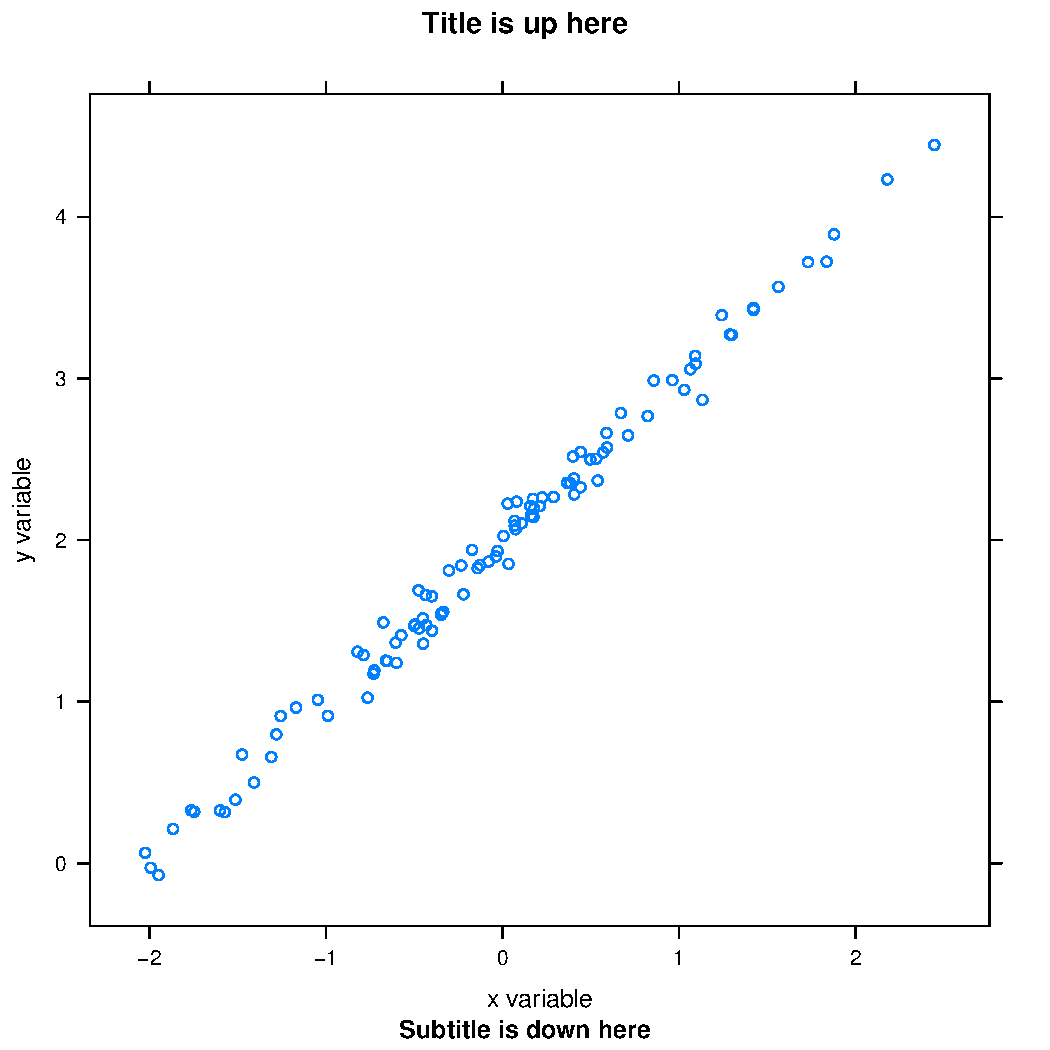
\includegraphics[width=\maxwidth]{figure/plot_echo-1} 

\end{knitrout}

Using \verb|echo=FALSE| will allow this next code chunk to be hidden,
  but the resulting plot still displays.

\begin{knitrout}
\definecolor{shadecolor}{rgb}{0.969, 0.969, 0.969}\color{fgcolor}
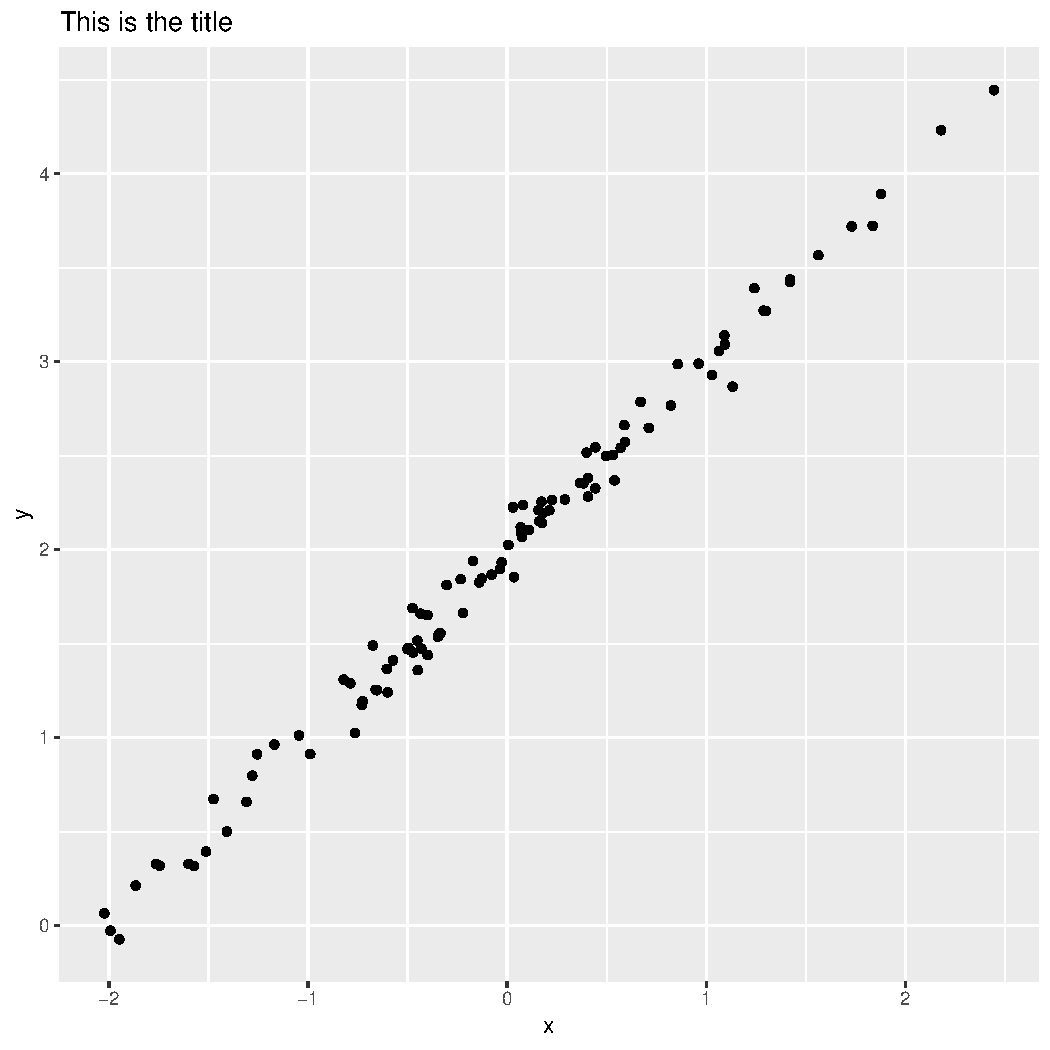
\includegraphics[width=\maxwidth]{figure/plot_hidden-1} 

\end{knitrout}

You can print an attractive table from R in a tabular environment.
Below are the first 10 observations from df.

% % tables are nicely produced using xtable and printing their output
% % look at help for ?xtable and ?print.xtable for many options
% <<texoutput, results='asis', echo=FALSE>>=
% library(xtable) # for tables
% xtab.out <- xtable(df[1:10,], digits=4)
% print(xtab.out, floating=FALSE, math.style.negative=TRUE)
% @

You can also write inline expressions,
  such as $\pi=3.1415927$, and \ensuremath{1.598673\times 10^{8}} is a big number.
The first values in the dataframe are $0.4429, 2.545$.

Equations will take a little practice, but will be beautiful.
The {\bf residual sum of squares (SS)} can be represented in many equivalent forms,
 %===============
\begin{eqnarray}
\label{eq:sse1}
  \textrm{SSE}(\hat{\beta})
    & = &
  \sum_{i=1}^{n} \{ y_{i} - (\hat{\beta}_{0} + \hat{\beta}_{1} x_{i 1} + \cdots + \hat{\beta}_{p} x_{ip}) \}^2
\\ %===
    & = &
  \sum_{i=1}^{n} \{ y_{i} - \hat{\mu}_{i} \}^2
\nonumber\\ %===
    & = &
  \sum_{i=1}^{n} \hat{e}_{i}^2
\nonumber\\ %===
\label{eq:epe}
    & = &
  \hat{e}^{\top} \hat{e}
\\ %===
    & = &
  (y - \hat{\mu})^{\top} (y - \hat{\mu})
\nonumber\\ %===
    & = &
  (y - \mathbf{X} \hat{\beta})^{\top} (y - \mathbf{X} \hat{\beta})
  .
\nonumber
\end{eqnarray}
 %===============
Equations \eqref{eq:sse1} and \eqref{eq:epe} are equivalent, and the equation
  reference numbers are connected to their labels in the equation array.


%%%%%%%%%%%%%%%%%%%%%%%%%%%%%%%%%%%%%%%%%%%%%%%%%%%%%%%%%%%%%%%%%%%%%%%%%%%%%%%%
\section{Section hierarchy}
These last few chunks below show the hierarchy of sections, subsections, etc. \ldots

Lorem ipsum dolor sit amet, consectetur adipisicing elit, sed do eiusmod tempor incididunt ut labore et dolore magna aliqua. Ut enim ad minim veniam, quis nostrud exercitation ullamco laboris nisi ut aliquip ex ea commodo consequat.

%%%%%%%%%%%%%%%%%%%%%%%%%%%%%%%%%%%%%%%%
\subsection{subsection}
Lorem ipsum dolor sit amet\ldots

Duis aute irure dolor in reprehenderit\ldots

%%%%%%%%%%%%%%%%%%%%
\subsubsection{subsubsection}
Lorem ipsum dolor sit amet\ldots

Duis aute irure dolor in reprehenderit\ldots

%%%%%%%%%%
\paragraph{paragraph}
Lorem ipsum dolor sit amet\ldots

Duis aute irure dolor in reprehenderit\ldots

%%%%%
\subparagraph{subparagraph}
Lorem ipsum dolor sit amet\ldots

Duis aute irure dolor in reprehenderit\ldots

%%%%%%%%%%%%%%%%%%%%%%%%%%%%%%%%%%%%%%%%%%%%%%%%%%%%%%%%%%%%%%%%%%%%%%%%%%%%%%%%
\section{OK, Go!}

Now you're ready (with practice) to create reproducible research!

%%%%%%%%%%%%%%%%%%%%%%%%%%%%%%%%%%%%%%%%%%%%%%%%%%%%%%%%%%%%%%%%%%%%%%%%%%%%%%%%
% Include code in an appendix, but just black-and-white
%   the development version of knitr allows you to do this
%   but not the current (2/2013) version
\appendix     % switches section numbers to letters

\section{Appendix, code}

Appendix stuff here.

\end{document}
%%%%%%%%%%%%%%%%%%%%%%%%%%%%%%%%%%%%%%%%%%%%%%%%%%%%%%%%%%%%%%%%%%%%%%%%%%%%%%%%

Any LaTeX after \end{document} is ignored.
R code chunks will still be processed.

%%%%%%%%%%%%%%%%%%%%%%%%%%%%%%%%%%%%%%%%%%%%%%%%%%
%
%  some examples of tables and graphics
%

The plot in Figure~\ref{fi:ed31b} on page~\pageref{fi:ed31b}
 \begin{figure}[hbtp]
\begin{center}
\includegraphics[scale=.7]{ed31b}
\caption{ed31b }
\label{fi:ed31b}
\end{center}
 \end{figure}

By Table~\ref{tab:31c} on page~\pageref{tab:31c}
 \begin{table}[hbtp]
\begin{center}
\caption{31c}
\label{tab:31c}
\begin{tabular}{l @{-} l @{=} r l}
\hline
\multicolumn{2}{c|}{Factors} & \multicolumn{2}{c}{Response Time} \\
$\bar{y}_{1.}$ & $\bar{y}_{2.}$ & 185.25 & $\star$ \\
\hline
\end{tabular}
\end{center}
 \end{table}

 %===============
\begin{eqnarray}
    & = &
\nonumber\\ %===
    & = &
\nonumber
\end{eqnarray}
 %===============

\begin{description}
   \item[]
\end{description}

1
